% *******************************************************************************
% * Copyright (c) 2008 by Elexis
% * All rights reserved. This document and the accompanying materials
% * are made available under the terms of the Eclipse Public License v1.0
% * which accompanies this distribution, and is available at
% * http://www.eclipse.org/legal/epl-v10.html
% *
% * Contributors:
% *    G. Weirich
% *
% *  $Id: update14.tex 4895 2009-01-02 07:16:49Z rgw_ch $
% *******************************************************************************

% !Mode:: "TeX:UTF-8" (encoding info for WinEdt)

\documentclass[a4paper]{scrartcl}

\usepackage{german}
\usepackage[utf8]{inputenc}
\usepackage{makeidx}
\usepackage[pdftex]{graphicx}
\DeclareGraphicsExtensions{.pdf,.jpg,.png}

\makeindex


\usepackage{floatflt}
\usepackage[]{hyperref}
\usepackage{color}

\begin{document}
\title{Elexis 1.4.0 - mise à niveau}
\author{G. Weirich}

\maketitle
\tableofcontents

\section{Quand et pour qui?}
La mise à niveau de la version 1.4 est conseillée à tous les utilisateurs de Elexis. \textbf{s.v.p veuillez consulter pour ce faire les instructions pour la mise à niveau à la page \pageref{update}}. Le meilleur moment pour la mise à niveau est lorsque vous avez facturé la majorité de tous les traitements, ce qui est normalement le cas au début d'une année.

\section{Quoi de neuf?}
A part de quelques corrections la version 1.4 contient quelques nouveautés :

\subsection{Nouveau Look}
Les Icons des premières versions de Elexis ont été cherchés selon besoin n'importe où et ceci se voyait dans le design. On a cherché d'améliorer et unifier pour la version 1.4 le design. (cf. Fig. \ref{fig:modern}). Celui qui préfère par contre l'ancien look peut à tout moment revenir à l'ancien design. \footnote{une surface adaptable selon gôut de l'utilisateur s'appelle en englais 'plaf' (pluggable look and feel)}.

\begin{figure}
%\begin{minipage} {0.5\textwidth}
    \center
  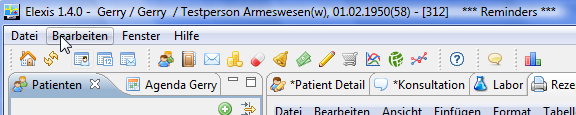
\includegraphics[width=0.7\textwidth]{modern}
  \caption{'Modern' Look}\label{fig:modern}
\end{figure}

%\end{minipage}
%\begin{minipage}{0.5\textwidth}
\begin{figure}
\center
  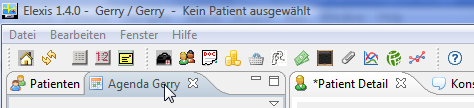
\includegraphics[width=0.7\textwidth]{classic}
  \caption{'Classic' Look}\label{fig:modern}
\end{figure}

\bigskip
On peut passer à un autre design en donnant à Elexis un paramètre de démarrage avec le plaf voulu :

\begin{itemize}
\item elexis - -plaf=rsc/plaf/modern  (nouveau look)
\item elexis - -plaf=rsc/plaf/classic (look classique)
\end{itemize}

Le look choisi reste enregistré jusqu'à ce qu'on veut passer explicitement à un design différent. Il n'est donc pas nécessaire d'introduire lors de chaque démarrage le paramètre.

\subsection{Adaptations au niveau du système de facturation}
\subsubsection{Proposition de facturation}
\begin{figure}
  % Requires \usepackage{graphicx}
  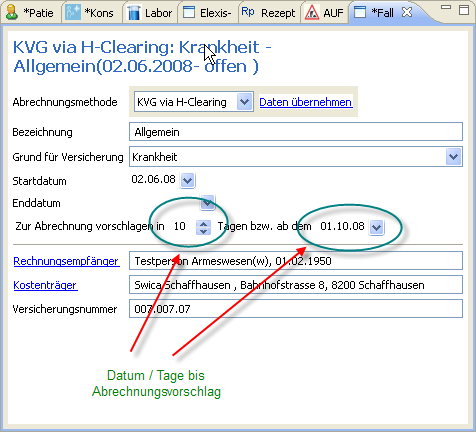
\includegraphics{abrvor1}\\
  \caption{Abrechnungsvorschlag}\label{fig:abrvor1}
\end{figure}

\begin{figure}
  % Requires \usepackage{graphicx}
  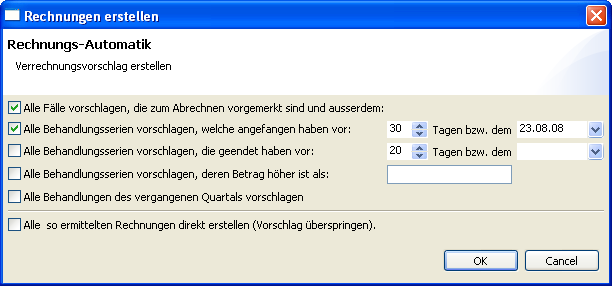
\includegraphics{abrvor2}\\
  \caption{Abrechnungsauswahl}\label{fig:abrvor2}
\end{figure}

Il est désormais possible de fixer dans les détails du cas (Fig. \ref{fig:abrvor1}), qu'un cas soit proposé à la facturation à partir d'une certaine date ou après un certain temps. Ceci permet par exemple lors de la garde de choisir que les cas soient facturés après 10 jours. Lors de la facturation on peut laisser faire une liste de tout les cas qui ont atteint l'échéance selon les conditions choisis.(Fig. \ref{fig:abrvor2}). Les champs pour les dates ont été développés pour qu'on puisse introduire soit le nombre de jours ou une date fixe.

En plus on peut facturer directement sans autres demandes de précisions ou possibilités de contrôle en cliquant sur le champs tout en bas.
\subsubsection{\%-suppléments et -rabais}
Autrefois pas traités de façon conforme au standard, ils ont été corrigés de sorte que par ex. la position 35.0020 soit calculée correctement avec un Scale-factor de -0.4 comme prestation à la hauteur des la prestation technique de la 'rubrique OP-I' correspondante.

\textbf{Important} Ce changement est la raison pour laquelle il est préférable de faire la mise à niveau 1.4 après fait la clôture des factures : Toutes les prestations qui contiennent des suppléments ou des rabais, lesquelles ont été calculés avec Elexis 1.3.x ne seront pas transférées correctement dans une facture faite sous Elexis 1.4. Si vous voulez pourtant faire la mise à niveau, même si vous avez encore des factures de ce genre ouvertes, il faudra ôter \textit{après} la mise à niveau 1.4 toutes les positions concernées et réintroduire de nouveau. Seulement par ce procédé la facturation se fera correctement.

\subsubsection{Details des prestations (page, prestations obligatoires)}
\begin{figure}
  % Requires \usepackage{graphicx}
  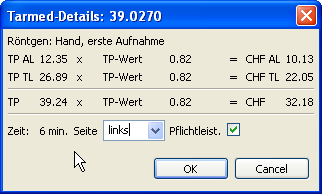
\includegraphics{tarmeddetail1}\\
  \caption{Detail zu Leistung}\label{fig:detail1}
\end{figure}

On peut désormais introduire des détails concernant des prestations calculées (Fig. \ref{fig:detail1}), en cliquant sur la prestation dans le champ de calcul à droite et en choisissant 'détails'. (Ceci n'est possible qu'en cas de prestation où des informations détaillées sont judicieuses). Ici on peut par ex. introduire droit ou gauche si c'est important ou on peut déclarer une prestation comme prestatio qui n'est pas obligatoirement prise en charge par l'assureur (par ex. une sonographie souhaitée par le patient mais qui n'était médicalement pas indiquée). 

\subsubsection{destinataire visible dans la View - détail de facturation}
Dans la View - détail de facturation on peut désormais voir le déstinataire de la facture. 

\subsection{médication fixe}
(Fig. \ref{fig:fixmedi})
\begin{figure}
  % Requires \usepackage{graphicx}
  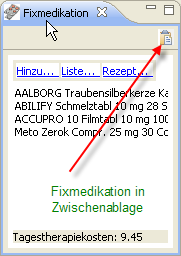
\includegraphics{fixmedi3}\\
  \caption{Fixmedikation}\label{fig:fixmedi}
\end{figure}

\begin{itemize}
\item Montre désormais les frais journaliers de thérapie (Ceci n'est possible que lorsque la taille de l'emballage et la fréquence de prise du médicament sont connues) 
\item Peut copier la médication dans le presse-papiers pour l'introduire ensuite par ex. dans une lettre ou dans le texte de la consultation.
\end{itemize}

\subsection{ordonnances}
Pour les ordonnances (comme jusqu'alors déjà dans la médication fixe) on peut désormais introduire des détails concernant la prescription en cliquant avec la touche droite sur un acticle (Fig. \ref{fig:einnahme1}).
\begin{figure}
  % Requires \usepackage{graphicx}
  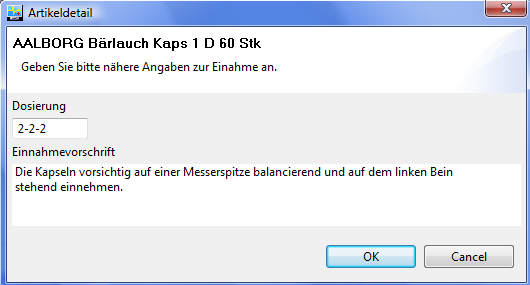
\includegraphics{einnahme1}\\
  \caption{Rezpet: Detailangaben}\label{fig:einnahme1}
\end{figure}

\subsection{sélecteur des contacts}
\begin{figure}
  % Requires \usepackage{graphicx}
  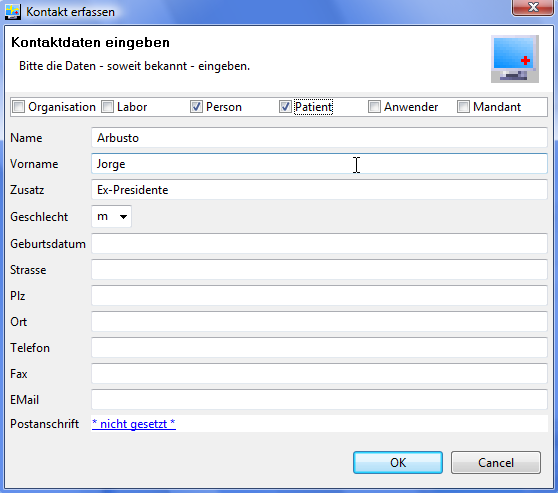
\includegraphics{kontakt}\\
  \caption{Kontakteingabe}\label{fig:kontakt}
\end{figure}

Lorsqu'un contact doit être choisi (par ex. pour les adresses des lettres) on peut désormais introduire directement un nouveau contact y inclus l'adresse.(Fig. \ref{fig:kontakt})

\subsection{importateur des résultats labo}
L'importateur des résultats de labo sur la base HL7 a été amélioré de sorte que les résultats histologiques et cytologiques apparaissent désormais dans un format lisible. 

\subsection{base}
Une noveauté que vous n'allez probablement pas remaquer à première vue mais qui contribue de façon importante à la stabilité et aux améliorations dans les détails : Elexis est désormais basé sur la version  actualisée 3.4 de Eclipse (Ganymede).

\subsection{divers}
Divers détails auquels on ne doit pas consacrer un chapitre spécifique ou qui ont déjà été mentionnés dans la documentation antérieure.

\section{instruction pour la mise à niveau}
\label{update}
\subsection{titulaire d'un contrat de maintenance et participant chez argoLEAD}
La mise à niveau à Elexis 1.4 ne se fait \textit{pas} automatiquement avec le logiciel de la mise à niveau mais doit être faite manuellement. Si vous avez un contrat de maintenance chez Elexis, vous ne devez rien faire : La mise à niveau fait partie du contrat de maintenance. Nous allons vous contacter pour accorder un rendez-vous de sorte que nous puissions faire cette installation.Si vous avez un contrat de maintenance chez une autre entreprise, veuillez vous informer si la mise à niveau est inclue dans le contrat de maintenance. Si vous êtes un participant du projet argoLEAD qui veut continuer à utiliser Elexis, nous allons, si vous le souhaitez, installer encore la mise à niveau 1.4 pour finir le Projet. (Ceci se fera soit par télémaintenance soit directement chez vous.) 

\subsection{Do it yourself}
N'installez la mise à niveau que si vous pouvez investir suffisamment du temps et si vous croyez pouvoir le faire vous-même en gardant toujours la possibilité en vue de pourvoir revenir en arrière sur l'ancienne version. En cas de doute nous vous conseillons de laisser faire ce travail par votre informaticien.

\medskip

Il est important d'éviter une installation mixte avec des plugins de la version 1.3 et d'autres de la version 1.4. veuillez considérer que les plugins de la version 1.3 ne seront souvent plus fonctionnels dans la version 1.4. Nous proposons de suivre la procédure suivante :

\begin{enumerate}
\item Si vous avez des plugins achetés chez Elexis, veuillez nous envoyer un mail à  support$@$elexis.ch avec une liste de vos plugins. Vous recevrez la mise à niveau 1.4 gratuitement. Si vous avez acheté des plugins chez un autre fournisseur, veuillez vous informer auprès de lui si vos plugins actuels fonctionnent dans Elexis 1.4 respectivement à quelles conditions la mise à niveau aura lieu.

\item Procédez à la mise à niveau seulement après la fermeture du cabinet quand vous aurez au moins une heure à disposition. Ne le faites seul que si vous êtes capables de revenir en arrière en réstaurant le système à l'état d'avant si jamais quelque chose ne marche pas. La mise à niveau doit se faire séparément sur tous les ordinateurs du réseau. L'utilisation mixte de Elexis 1.3.x et 1.4.x sur la même base de données n'est pas possible.
\item Nous vous conseillos vivement de faire un Backup complet de la base de données et des fichiers d'installation de Elexis. \textbf{Surtout ne sautez pas ce pas car il s'agit de la seule possibilité de revenir en arrière lors d'un problème avec la mise à jour }
\item Téléchargez l'installateur de Elexis 1.4 pour votre système d'exploitation chez www.elexis.ch.
\item Changez le nom du dossier actuel. Si Elexis est installé à c:$\backslash$Programme$\backslash$elexis, nommez ce fichier comme suit : c:$\backslash$Programme$\backslash$elexis-alt. \textbf{Important}: Vous ne devez donc pas copier mais changer le nom du fichier. Le fichier c:$\backslash$Programme$\backslash$elexis ne doit finalement plus exister.
\item Demarrez (Windows)réspectivement décompactez (Linux, Mac) l'installateur et choisissez comme lieu d'installation de Elexis le même endroit où Elexis était déjà installé.w an dem Elexis vorher installiert war (donc selon l'exemple d'avant c:$\backslash$Programme$\backslash$elexis). De cette manière on garanti que toutes les références internes et externes restent en vigeur de sorte que rien ne doit être configuré de nouveau.  
\item Startez Elexis d'abord que sur un ordinateur et aiez un peu de patience : Puisque la base de données sera réorganisée, le premier démarrage pourra durer jusqu'à 10 minutes avant que la fenêtre de Elexis apparaisse. 
\item Ensuite, vous pouvez démarrer Elexis sur toutes les ordinateurs du réseau. Testez surtout aussi si vous pouvez imprimer des ordonnances pour ne pas constater le problème le lendemain lorsque tout devrait être prêt. 
\item Si tout fonctionne normalement, veuillez installer vos plugins supplémentaires  mais comme déjà mentionné que dans une version cértifiée 1.4. .
\end{enumerate}

\subsubsection{Si quelque chose n'a pas marché}
Comme toujours avec les ordinateurs on ne peut jamais garantir que toutes les choses se passent bien chez tout le monde. Pour cette raison on a besoin de la possibilité de pouvoir revenir sur l'ancienne version pour pouvoir continuer le travail. Puisque Elexis 1.4 change quelque peu la base de données aucun client qui est resté sur la version 1.3. ne pourra fonctionner. Ceci provoquera lors du démarrage un message d'erreur. Vous devez donc procéder de façon suivante :
\begin{enumerate}
\item Fermez Elexis sur tous les ordinateurs du réseau
\item faites un 'Restore' du Backup que vous avez fait avant la mise à niveau 1.4. pour réinstaller la base de donnée de la version 1.3.x.
\item Effacez les répertoires de Elexis dans tous les ordinateurs (ou changez le nom par ex. à 'elexis-1.4' ).
\item Changez les répertoires nommés 'elexis-old' en 'elexis'.

\end{enumerate}
Par la suite Elexis marche de nouveau dans l'ancienne version qui existait avant la mise à niveau. Appelez votre informaticien pour faire votre mise à niveau à un autre moment. 

\subsection{Utilisateur Beta}
Même si vous avez déjà utilisé une beta-version 1.4 vous devez pourtant télécharger l'installateur complet et ensuite l'installer, comme mentionné ci-dessus, dans un répertoire vide. Une mise à niveau simple de 1.4 beta à 1.4 provoquera probablement des problèmes entre dautre avec des plugins qui ne fonctionneront plus. 

\section{Perspective}
Entre temps on peut considerer Elexis  comme logiciel qui a muri et qui peut être utilisé de façon professionnelle.Nous entrons actuellement dans une phase de réalignement et de développement fonctionnel. On a constaté que la complexité de la matière du 'dossier électronique' exîge une maintenance et que pour une maintenance professionnelle il faudra aussi avoir la structure d'une organisation professionnelle qui nécessite une certaine base de financement. 

Le noyeau de Elexis et les plugins qui seront nécessaires pour un dossier électronique simple et rapidement disponsible resteront toujours OpenSource et librement accessibles. Par contre les contrats de maintenance devraient gagner en attractivité de sorte que le besoin de maintenance qui augmente avec la quantité des utilisateurs  pourra être financé. Les capacités du petit groupe de developpeurs de Elexis devraient pouvoir être utilisées pour le développement du produit et non seulement pour la maintenance. L'idée est de faire profiter doublement l'utilisateur qui paye un contrat de maintenance annuelle : D'un côté il recevra certaines prestations supplémentaires en comparaison à l'utilisateur sans contrat de maintenance et de l'autre côté il participe ainsi au développement du logiciel ce qui le laisse en profiter plus rapidement. En plus il sera possible que l'utilisateur de Elexis puisse acheter des actions de l'entreprise qui s'est formé autour ce logiciel, chose qui lui donnera certains avantages en comparaison à l'utilisateur sans contrat. 
\medskip

Elexis 2.0 est en voie de développement et contiendra toute une somme de nouveautés. Si vous voulez vous tenir au courrant vous avez les possibilités suivantes : Soit vous vous renseignez de temps en temps sur la Website (http://www.elexis.ch) ou dans le  forum de elexis(http://www.elexis-forum.ch\footnote{Vous pouvez aussi vous abonner au forum d'un RSS-Feed, pour que vous soyez toujours informés automatiquement des nouveautés.}) Vous pouvez aussi vous mettre sur la Mailing-List ce qui vous permet d'être informé automatiquement concernant les nouveautés importantes. (un mail à support$@$elexis.ch suffit pour s'inscrire ).

\medskip

Vos questions, suggestions et remarques sont bienvenus chez support$@$elexis.ch et nous essayerons comme toujours de vous répondre au plus vite possible.

\end{document}
